%Die Angabe des schlauen Spruchs auf diesem Wege funtioniert nur,
%wenn keine Änderung des Kapitels mittels den in preambel/chapterheads.tex
%vorgeschlagenen Möglichkeiten durchgeführt wurde.
\chapter{Evaluation of results}
\label{chap:chapter6}
%\vspace{-3cm}
%\vspace{2cm}
This chapter presents results of classification using experimental setup described in chapter~\ref{chap:chapter6}. The term \emph{Classification accuracy} of a class used in chapter is defined as,

\[ \begin{array}{ll} accuracy(r_i) = \frac{\mbox{Samples correctly predicted as $r_i$}}
								{\mbox{Total samples with label $r_i$}}
							\times 100 & 
							\forall \,r_i \in \{\mbox{\texttt{P,I,T}}\} 
	\end{array}\]

Where, $r$ is the label of test sample $x=\{\boldsymbol{x},r\}$.

In the presented evaluation, cross-validation accuracy is also noted for each set of experiments, as this is value of accuracy during self-validation of much larger training set.

In the first part analyzes classification efficiency after grid search for optimal values of $C$ and $\gamma$, but does not consider any other optimization, detailed account of results are presented for each kernel type available in \texttt{LIBSVM}. Second part improvises the first, and results are noted after optimization of so-called \emph{class-weights}. Third part explores two possibilities -that of using one  of using single prediction model for predicting all types of circuits, and second to extrapolating known model to predict new circuit types. The last part tries to evaluate impact on yield and quality of final product after application of suggested method.

\section{Classification of permanent faults}
\label{sec:wp}
Consider a special case, where $\epsilon = Test Runs$. In our classification problem this can mean,
\begin{enumerate}
  \item It is a permanent fault.
  \item A rare case of highly repetitive intermittent fault, and can be said to be \enquote{critical}.
  \item An extremely rare transient fault, as it happened at the same location and for same input test pattern, in all of the test runs.
\end{enumerate}

In the other direction, for permanent faults $\epsilon = Test Runs$ holds true, except a rare possibility that transient noise affects all the test patterns, which have resulted in failure at POs, in at least one of test runs. This is also an extremely rare possibility. Hence we assume that, a fault is permanent if and only if $\epsilon = Test Runs$.

If we go back to section~\ref{sec:secfs} and observe the plot for $\epsilon$ in figure~\ref{fig:epsilonp45k}, we can observe our assumption to be fairly accurate. Hence if we do a slight modification in our experimental setup and already remove faults where $\epsilon = Test Runs$, and classify them as permanent faults, we can achieve 100\% permanent fault classification, and we would be left with a binary classification problem between transient and intermittent faults. 

\section{Classification without class-weight optimization}
First set of experiments consist of evaluation of accuracy levels without assigning class weights \emph{i.e.} class-weights are assumed to be \{1,1,1\} for permanent, intermittent and transient faults respectively. The experiments are carried out for variety of circuits ranging from simple p45k to highly complex p295k. The experiments are repeated for each type of kernel provided by \texttt{LIBSVM}. 

This set of experiments consist of two rounds each for each kernel, first one includes permanent faults in sample population, the other one without considering them. A round with permanents is carried out only to evaluate change in accuracy levels of classification.

\subsection{Linear Kernel}
Accuracy of SVM using linear kernel is summarized in table~\ref{tab:linwp} with considering permanent faults in sample population, and the same without considering permanents is summarized in table~\ref{tab:linwop}.
\begin{table}[h]

	\captionsetup{justification=centering}
\begin{tabular}{ccccccc}
\hline
\multicolumn{1}{c}{\multirow{3}{*}{Circuit}} & \multicolumn{6}{c}{Accuracy (\%)}\\ \cline{2-7} 
\multicolumn{1}{c}{}                         & \multicolumn{1}{c}{\multirow{2}{*}{Cross-validation}} & \multicolumn{2}{c}{Permanent} & \multicolumn{2}{c}{Intermittent} & \multicolumn{1}{c}{\multirow{2}{*}{Transient}} \\ \cline{3-6}
                                             &                                                       & w/o noise     & with noise    & w/o noise      & with noise      &                                                \\ \hline
p45k                                         & 90.14                                                 & 87.50         & 87.50         & 77.50          & 64.58           & 93.90                                          \\
p100k                                        & 87.38                                                 & 100           & 100           & 80.95          & 57.14           & 95.91                                          \\
p141k                                        & 83.89                                                 & 98.21         & 98.21         & 61.90          & 57.14           & 100                                            \\
p267k                                        & 85.12                                                 & 100           & 100           & 55.00          & 52.50           & 100                                            \\
p279k                                        & 89.52                                                 & 98.30         & 96.61         & 78.94          & 52.50           & 89.79                                          \\
p295k                                        & 89.84                                                 & 100           & 100           & 81.39          & 65.11           & 100   \\
\hline                                        
\end{tabular}
\caption {Classification accuracy for linear kernel}
\label{tab:linwp}
\end{table}

In both cases, with and without permanent faults, it can be observed that, permanent faults are being relatively accurately being classified and background transient noise seems to have almost no effect on classification accuracy of permanent faults. Intermittent faults in both cases have relatively low accuracy levels and tend to deteriorate severely in presence of transient noise. 


\begin{table}[h]
\captionsetup{justification=centering}
\begin{tabular}{ccccc}
\hline
\multirow{3}{*}{Circuit} & \multicolumn{4}{c}{Accuracy (\%)}\\ \cline{2-5} 
                         & \multirow{2}{*}{Cross-validation} & \multicolumn{2}{c}{Intermittent} & \multirow{2}{*}{Transient} \\ \cline{3-4}
                         &                                   & w/o noise      & with noise      &                            \\ \hline
p45k                     & 87.81                             & 72.91          & 70.08           & 97.95                      \\
p100k                    & 81.43                             & 69.05          & 59.52           & 97.96                      \\
p141k                    & 84.13                             & 78.57          & 76.19           & 100                        \\
p267k                    & 77.09                             & 80.00          & 55.00           & 100                        \\
p279k                    & 84.65                             & 78.94          & 52.63           & 91.83                      \\
p295k                    & 89.17                             & 90.69          & 81.39           & 100           \\
\hline            
\end{tabular}
\caption {Classification accuracy for linear kernel, without permanent faults}
\label{tab:linwop}
\end{table}

After removing permanents from the sample population, classification accuracies are observed to improve, with an exception of p100k. However, accuracy levels are observed to increase for intermittents with noise even in the case of p100k. Classification accuracy of transient faults has also increased. Cross-validation accuracy levels have decreased, as large chuck of correctly classified data in earlier case was permanent faults. Comparatively lower accuracy levels for intermittent faults and almost 100\% classification rate for transients suggests that, linear kernel is more biased towards transient faults.

\subsection{Polynomial Kernel}
\begin{table}[h]

	\captionsetup{justification=centering}
\begin{tabular}{ccccccc}
\hline
\multirow{3}{*}{Circuit} & \multicolumn{6}{c}{Accuracy (\%)}\\ \cline{2-7} 
                         & \multirow{2}{*}{Cross-validation} & \multicolumn{2}{c}{Permanent} & \multicolumn{2}{c}{Intermittent} & \multirow{2}{*}{Transient} \\ \cline{3-6}
                         &                                   & w/o noise     & with noise    & w/o noise      & with noise      &                            \\ \hline
p45k                     & 90.92                             & 87.50         & 89.58         & 68.75          & 70.83           & 83.67                      \\
p100k                    & 89.70                             & 100           & 97.82         & 69.04          & 66.66           & 93.87                      \\
p141k                    & 87.94                             & 100           & 100           & 73.80          & 71.42           & 95.00                      \\
p267k                    & 87.34                             & 100           & 96.55         & 82.50          & 60.00           & 85.71                      \\
p279k                    & 91.42                             & 98.30         & 96.55         & 81.57          & 73.68           & 91.83                      \\
p295k                    & 90.78                             & 100           & 98.21         & 76.09          & 72.09           & 95.91      \\
\hline                                                     
\end{tabular}
\caption {Classification accuracy for polynomial kernel}
\label{tab:polywp}
\end{table}

Accuracy of SVM using polynomial kernel is summarized in table~\ref{tab:polywp} with considering permanent faults in sample population, and the same without considering permanents is summarized in table~\ref{tab:polywop}.

Accuracy of classification of permanent faults, without noise in case of polynomial kernel is observed to be even higher than linear kernel. For permanents with noise, classification rates are almost similar. Intermittent faults with permanents in first round, without noise are deteriorating in some cases, while improving significantly in others. With noise, however, accuracy of intermittent fault classification is improved. Classification accuracy of transient faults is decreased as compared to linear kernel.

\begin{table}[h]
\captionsetup{justification=centering}
\begin{tabular}{ccccc}
\hline
\multirow{3}{*}{Circuit} & \multicolumn{4}{c}{Accuracy (\%)}\\ \cline{2-5} 
                         & \multirow{2}{*}{Cross-validation} & \multicolumn{2}{c}{Intermittent} & \multirow{2}{*}{Transient} \\ \cline{3-4}
                         &                                   & w/o noise      & with noise      &                            \\ \hline
p45k                     & 87.81                             & 81.25          & 72.91           & 87.76                      \\
p100k                    & 85.00                             & 78.57          & 66.66           & 89.79                      \\
p141k                    & 85.57                             & 80.95          & 76.19           & 100                        \\
p267k                    & 81.38                             & 82.50          & 72.50           & 93.87                      \\
p279k                    & 85.57                             & 78.94          & 73.68           & 93.87                      \\
p295k                    & 92.28                             & 93.02          & 86.04           & 93.87                      \\
\hline
\end{tabular}
\caption {Classification accuracy for polynomial kernel, without permanent faults}
\label{tab:polywop}
\end{table}

In second round, after removing permanents, a huge improvement in accuracy of intermittent faults is observed as compared to the first round. The results are also better than those for linear kernel.  A marginal improvement in transient fault classification accuracy is also observed as compared to the first round. However, overall figures for transients are lower than those for linear kernel. Observations suggest that, polynomial kernel is slightly biased towards intermittents.


\subsection{RBF Kernel}

Accuracy of SVM using Radial Basis Function (RBF) kernel is summarized in table~\ref{tab:rbfwp} with considering permanent faults in sample population, and the same without considering permanents is summarized in table~\ref{tab:rbfwop}.

\begin{table}[h]

	\captionsetup{justification=centering}
\begin{tabular}{ccccccc}
\hline
\multirow{3}{*}{Circuit} & \multicolumn{6}{c}{Accuracy (\%)}\\ \cline{2-7} 
                         & \multirow{2}{*}{Cross-validation} & \multicolumn{2}{c}{Permanent} & \multicolumn{2}{c}{Intermittent} & \multirow{2}{*}{Transient} \\ \cline{3-6}
                         &                                   & w/o noise     & with noise    & w/o noise      & with noise      &                            \\ \hline
p45k                     & 91.21                             & 100           & 100           & 66.66          & 64.58           & 91.83                      \\
p100k                    & 87.36                             & 100           & 100           & 64.28          & 61.94           & 93.87                      \\
p141k                    & 88.63                             & 100           & 100           & 73.80          & 71.42           & 93.87                      \\
p267k                    & 87.27                             & 100           & 98.27         & 80.00          & 72.50           & 93.87                      \\
p279k                    & 89.52                             & 98.30         & 96.55         & 78.92          & 71.05           & 93.87                      \\
p295k                    & 91.00                             & 100           & 100           & 79.06          & 74.41           & 95.91                     \\
\hline                                                     
\end{tabular}
\caption {Classification accuracy for RBF kernel}
\label{tab:rbfwp}
\end{table}
Classification rates for permanent faults, with and without noise, are higher for RBF kernel as compared to others. Like in other cases, injection of transient noise has affected accuracy of intermittent fault classification, significantly. Accuracy figures for both, intermittent faults with and without noise, are lower as compared to previous two kernels. Transient fault classification accuracy shows marginal improvement over polynomial kernel, but is still lower than the linear kernel.

Intermittent fault classification accuracy is increased for simpler circuits, but shows no change for more complex circuits. However, for intermittent faults injected with noise, accuracy is improved as compared to the first round, but is till lower than other kernel types. A slight increase in transient fault classification accuracy is also observed. 

A notable observation in case of RBF kenrel is its comparatively higher cross-validation accuracy figures and lower test set classification accuracy, an indication that the kernel may be overfitting.

\begin{table}[h]
	\captionsetup{justification=centering}
\begin{tabular}{ccccc}
\hline
\multirow{3}{*}{Circuit} & \multicolumn{4}{c}{Accuracy (\%)}                                                                 \\ \cline{2-5} 
                         & \multirow{2}{*}{Cross-validation} & \multicolumn{2}{c}{Intermittent} & \multirow{2}{*}{Transient} \\ \cline{3-4}
                         &                                   & w/o noise      & with noise      &                            \\ \hline
p45k                     & 87.56                             & 77.08          & 70.83           & 91.83                      \\
p100k                    & 83.33                             & 78.57          & 64.28           & 89.79                      \\
p141k                    & 86.53                             & 83.33          & 80.95           & 100                        \\
p267k                    & 80.19                             & 82.50          & 70.00           & 92.34                      \\
p279k                    & 85.64                             & 78.92          & 76.31           & 95.91                      \\
p295k                    & 85.64                             & 79.06          & 76.31           & 95.91  						  \\
\hline
\end{tabular}
\caption {Classification accuracy for RBF kernel, without permanent faults}
\label{tab:rbfwop}
\end{table}


\subsection{Sigmoid Kernel}

Accuracy of SVM using Radial Basis Function (RBF) kernel is summarized in table~\ref{tab:sigwp} with considering permanent faults in sample population, and the same without considering permanents is summarized in table~\ref{tab:sigwop}.

Again, the permanent fault classification rates for permanent faults is fairly high for sigmoid kernel also. The Intermittent fault classification accuracy is comparatively low (except p100k) despite high cross validation accuracy. This coupled with high transient fault classification accuracy indicate that, sigmoid kernel is biased towards transient faults. This has also resulted in degradation of accuracy levels when intermittents were injected with transient noise.

\begin{table}[h]

	\captionsetup{justification=centering}
\begin{tabular}{ccccccc}
\hline
\multirow{3}{*}{Circuit} & \multicolumn{6}{c}{Accuracy (\%)}\\ \cline{2-7} 
                         & \multirow{2}{*}{Cross-validation} & \multicolumn{2}{c}{Permanent} & \multicolumn{2}{c}{Intermittent} & \multirow{2}{*}{Transient} \\ \cline{3-6}
                         &                                   & w/o noise     & with noise    & w/o noise      & with noise      &                            \\ \hline
p45k                     & 89.55                             & 97.50         & 97.50         & 77.08          & 60.41           & 95.91                      \\
p100k                    & 85.08                             & 100           & 100           & 95.23          & 52.38           & 71.42                      \\
p141k                    & 84.17                             & 100           & 100           & 57.14          & 57.14           & 100                        \\
p267k                    & 82.46                             & 100           & 98.27         & 42.50          & 42.50           & 100                        \\
p279k                    & 89.29                             & 98.30         & 96.55         & 81.57          & 52.63           & 87.76                      \\
p295k                    & 85.09                             & 98.21         & 98.21         & 69.76          & 65.11           & 100                       \\
\hline                                                     
\end{tabular}
\caption {Classification accuracy for sigmoid kernel}
\label{tab:sigwp}
\end{table}

The kernel became more biased towards transients when permanent fault examples were removed from sample population. Transient fault classification accuracy was observed to increase to near 100\%. However, intermittent classification accuracy also increased at the same time, with and without transient noise.

\begin{table}[h]
\captionsetup{justification=centering}
\begin{tabular}{ccccc}
\hline
\multirow{3}{*}{Circuit} & \multicolumn{4}{c}{Accuracy (\%)}                                                                 \\ \cline{2-5} 
                         & \multirow{2}{*}{Cross-validation} & \multicolumn{2}{c}{Intermittent} & \multirow{2}{*}{Transient} \\ \cline{3-4}
                         &                                   & w/o noise      & with noise      &                            \\ \hline
p45k                     & 84.46                             & 68.75          & 60.41           & 100                        \\
p100k                    & 80.00                             & 81.39          & 52.38           & 100                        \\
p141k                    & 80.04                             & 78.57          & 73.80           & 100                        \\
p267k                    & 75.17                             & 75.00          & 55.00           & 100                        \\
p279k                    & 83.41                             & 81.57          & 52.63           & 91.83                      \\
p295k                    & 92.28                             & 93.02          & 86.04           & 91.83                     \\
\hline
\end{tabular}
\caption {Classification accuracy for sigmoid kernel, without permanent faults}
\label{tab:sigwop}
\end{table}

This set of experiments show that the relative accuracy levels for fault classification actually increase if the sample population and test data is pre-screened for permanents faults. Hence for the rest of the evaluation,  all experiments are done by considering that sample population consists of intermittent and transient faults only.

\subsection{Analysis of intermittent fault classification}
\label{sec:wp:intanalysis}
The first set of experiments reveal that the classification accuracy for intermittent faults comparatively low as compared to other fault types. Hence more detailed analysis is done, which can provide some hints about the improvement of intermittent fault classification accuracy. First, an analysis is done about how fault activation rates might be affecting classification accuracy. Table~\ref{tab:intdetail} summarizes the result of this analysis and it notes accuracy results for different intermittent fault activation rates, for examples in the test dataset. For this analysis, a subset of circuits were analyzed using all four kernels of \texttt{LIBSVM}.

\begin{table}[h]
\captionsetup{justification=centering}
\resizebox{\textwidth}{!}{%
\begin{tabular}{cccccccc}
\hline
\multirow{3}{*}{Circuit} & \multirow{3}{*}{Kernel} & \multicolumn{6}{c}{Classification accuracy (\%)}\\ \cline{3-8} 
                         &                         & \multicolumn{3}{c}{Intermittent faults without noise} & \multicolumn{3}{c}{Intermittent faults with noise} \\ \cline{3-8} 
                         &                         & rate = 0.1    & rate = 0.01    & rate = 0.001   & rate = 0.1   & rate = 0.01   & rate = 0.001  \\ \hline
\multirow{4}{*}{p141k}   & linear                  & 100           & 81.25          & 25.00          & 100          & 75.00         & 25.00         \\
                         & polynomial              & 100           & 81.25          & 37.5           & 100          & 75.00         & 25.00         \\
                         & RBF                     & 100           & 81.25          & 50.00          & 100          & 81.25         & 37.5          \\
                         & sigmoid                 & 100           & 81.25          & 25.00          & 100          & 68.75         & 25.00         \\
\hline
\multirow{4}{*}{p267k}   & linear                  & 94.73         & 82.35          & 20.00          & 89.47        & 35.29         & 0.00          \\
                         & polynomial              & 94.73         & 88.23          & 20.00          & 94.73        & 64.70         & 20.00         \\
                         & RBF                     & 94.73         & 88.2           & 20.00          & 94.73        & 58.82         & 20.00         \\
                         & sigmoid                 & 94.73         & 70.58          & 20.00          & 89.47        & 35.29         & 0.00          \\

\hline
\multirow{4}{*}{p295k}   & linear                  & 100           & 88.23          & 77.77          & 100          & 88.23         & 33.33         \\
                         & polynomial              & 100           & 94.11          & 77.77          & 100          & 100           & 33.33         \\
                         & RBF                     & 100           & 94.117         & 77.77          & 100          & 100           & 33.33         \\
                         & sigmoid                 & 100           & 88.23          & 77.77          & 100          & 76.47         & 22.22     	\\
\hline   
\end{tabular}
}
\caption{Accuracy of intermittent fault classification for different fault rates}
\label{tab:intdetail}
\end{table}

The analysis shows that, accuracy levels are fairly high for high fault activation rates of intermittent faults, but go on deteriorating for lower values of fault activation rates. The main reason this behavior is that, at lower fault activation rates of $10^{-3}$, the behavior of transient faults (activation rates for which are $10^{-2}$ to $10^{-4}$) matches behavior of intermittents, and the learning algorithm fails to separate both from each other. This suggests that, instances where intermittent failures occurred only once and did not repeat themselves, are not able to convey enough information in their extracted features. To further elaborate this, accuracy analysis for the same circuits from table~\ref{tab:intdetail} is done by removing those intermittent faults from the test set, whose reproducibility ($\epsilon$) is less than one. The results of this analysis are presented in table~\ref{tab:intsweep}.

\begin{table}[h]
\begin{tabular}{ccccc}
\hline
\multirow{3}{*}{Circuit} & \multirow{3}{*}{Kernel} & \multicolumn{3}{c}{Classification accuracy (\%)}              \\ \cline{3-5} 
                         &                         & \multicolumn{2}{c}{Intermittent} & \multirow{2}{*}{Transient} \\ \cline{3-4}
                         &                         & w/o noise      & with noise      &                            \\ \hline
\multirow{4}{*}{p141k}   & linear                  & 100            & 100             & 100                        \\
                         & polynomial              & 100            & 100             & 100                        \\
                         & RBF                     & 100            & 100             & 100                        \\
                         & sigmoid                 & 100            & 100             & 100                        \\
\hline
\multirow{4}{*}{p267k}   & linear                  & 100            & 100             & 100                        \\
                         & polynomial              & 100            & 100             & 93.87                      \\
                         & RBF                     & 100            & 100             & 95.91                      \\
                         & sigmoid                 & 100            & 100             & 100                        \\
\hline
\multirow{4}{*}{p295k}   & linear                  & 100            & 100             & 100                        \\
                         & polynomial              & 100            & 100             & 93.87                      \\
                         & RBF                     & 100            & 100             & 91.83                      \\
                         & sigmoid                 & 100            & 100             & 91.83                     \\
\hline
\end{tabular}
\caption{Improvement in accuracy levels after removing intermittents with $\epsilon = 1$}
\label{tab:intsweep}
\end{table}

The analysis from table~\ref{tab:intsweep} shows that, if we remove such data from the test set, classification of intermittent faults is accurate. Accuracy of transient fault classification remains the same as the same classifier model and the same test dataset for transient faults is used as earlier experiments.

\section{With class-weight optimization}
\label{sec:ww}
The other possibility than the one suggested in the section~\ref{sec:wp:intanalysis} is to balance the training dataset. An unbalanced dataset is a possibility in our case, as we have set a tolerance of $\pm$ 75 examples, as explained in section~\ref{sec:gsp:configuration}. Class-weights are used while training the SVM by adding a penalty to samples of particular class, compensate for the unavailability of enough positive examples for that class. To other way to look at this, is that, when we apply class-weights, we deliberately underfit examples of those particular classes.

\texttt{LIBSVM} provides a functionality to adjust individual class weights, to bias classification towards a specified class using \texttt{-wi} switch. We can use this functionality to:
\begin{itemize}
  \item Fine-tune $C$ values for optimal classification. This way we can have a classifier which can separate most of examples in dataset.
  \item Optimize classifier for classifying one type of faults more accurately than the other.This is particularly useful the user is more interested in optimizing for the quality, then he may wish to reject all chips with a slightest possibility of intermittent failure. In this case classifier can be optimized for classifying intermittent faults more accurately. On the other hand, if user wants to optimize for quality, classifier can be tuned to classify transient faults more accurately.
\end{itemize}  

Table~\ref{tab:optp267k} shows accuracy values, when optimizations mentioned above are performed.

\begin{table}[h]
\captionsetup{justification=centering}
\begin{tabular}{cccccc}
\hline
\multirow{3}{*}{Kernel}     & \multirow{3}{*}{Optimization Criterion} & \multirow{3}{*}{Class-weights \{\texttt{I,T}\}} & \multicolumn{3}{c}{Classification accuracy (\%)}              \\ \cline{4-6} 
                            &                                         &                                                   & \multicolumn{2}{c}{Intermittent} & \multirow{2}{*}{Transient} \\ \cline{4-5}
                            &                                         &                                                   & w/o noise      & with noise      &                            \\ \hline
\multirow{3}{*}{linear}     & Intermittent                            & \{1.5,1\}                                         & 100            & 100             & 22.44                      \\
                            & Transient                               & \{1,1\}                                           & 80.00          & 55.00           & 100                        \\

                            & All                               & \{1.9,1.8\}                                           & 72.5          & 67.5           & 95.91                        \\
\hline
\multirow{3}{*}{polynomial} & Intermittent                            & \{1.85,1.05\}                                     & 97.50          & 80.00           & 20.00                      \\
                            & Transient                               & \{1.3,1.95\}                                      & 82.50          & 67.50           & 97.95                      \\

                            & All                               & \{1.9,1.25\}                                           & 95.00          & 78.00           & 77.5                        \\
\hline
\multirow{3}{*}{RBF}        & Intermittent                            & \{1.75,1.15\}                                     & 95.00          & 72.50           & 89.79                      \\
                            & Transient                               & \{1.2,1.3\}                                       & 72.50          & 70.00           & 95.91                      \\

                            & All                               & \{1,1\}                                           & 82.50          & 70.00           & 92.34                        \\
\hline
\multirow{3}{*}{sigmoid}    & Intermittent                            & \{1.7,1.1\}                                       & 85.00          & 77.50           & 65.30                      \\
                            & Transient                               & \{1.9,1.8\}                                       & 82.5           & 57.5            & 100                       \\

                            & All                               & \{1.7,1.75\}                                           & 82.50          & 47.00           & 100                        \\
\hline
\end{tabular}
\caption{Accuracy after class-weight optimization for p267k}
\label{tab:optp267k}
\end{table}

To find out optimal values of weights in case of optimization for intermittent and transient faults, an exhaustive search of combinations of class-weights for \texttt{I} and \texttt{T} classes is performed. For experimental purpose, a limited search of region [1,2] with steps of 0.5 for combinations of class-weights is performed. Heat-maps for this search are shown in figure~\ref{fig:heatmap} for p267k.

Optimization for \enquote{All} labels is done by considering weights corresponding to highest cross-validation accuracy. After class-weight optimization, accuracy levels are observed to be improved as compared to the same analysis done in section~\ref{sec:wp}.


\begin{figure}
        \centering
			\captionsetup{justification=centering}
        \begin{subfigure}[h]{0.45\linewidth}
                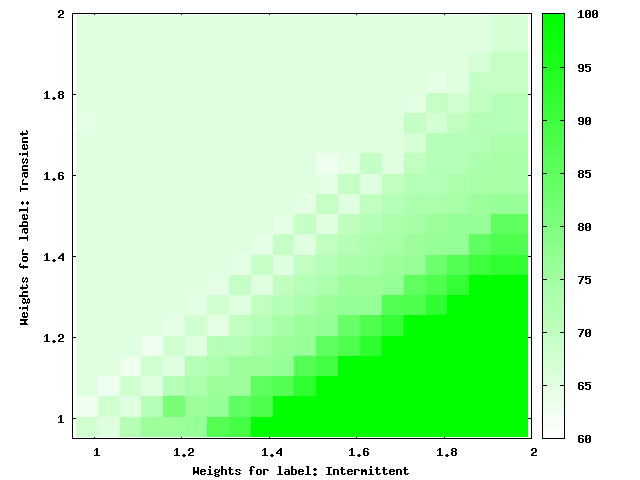
\includegraphics[scale=0.25]{figures/lin256i.png}
                \caption{Intermittent fault accuracy, linear kernel}
        \end{subfigure}
        \begin{subfigure}[h]{0.45\linewidth}
                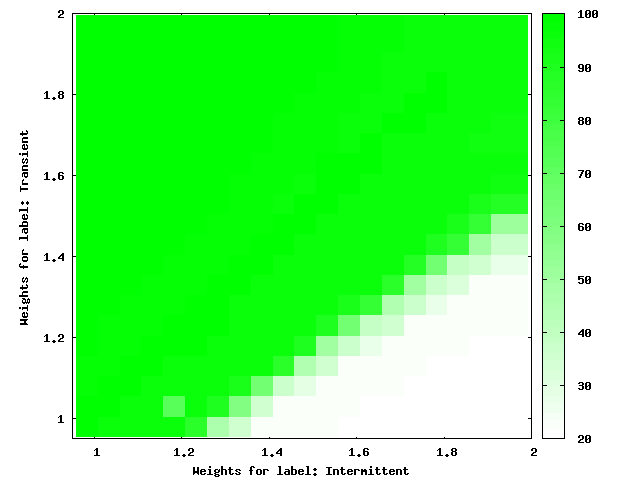
\includegraphics[scale=0.25]{figures/lin256t.png}
                \caption{Transient fault accuracy, linear kernel}
        \end{subfigure}

			\begin{subfigure}[h]{0.45\linewidth}
                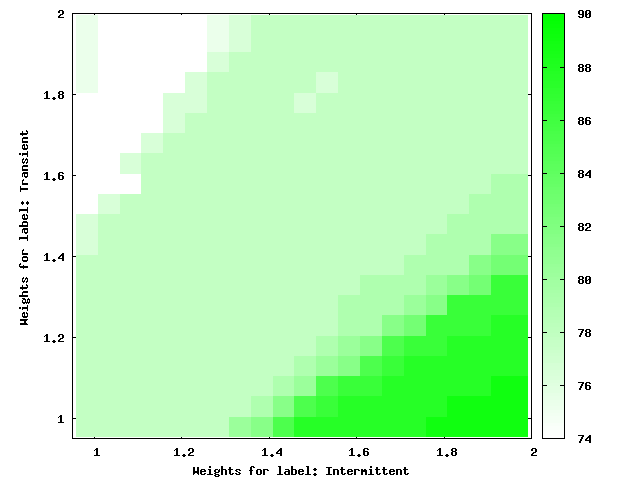
\includegraphics[scale=0.25]{figures/poly256i.png}
                \caption{Intermittent fault accuracy, polynomial kernel}
        \end{subfigure}
        \begin{subfigure}[h]{0.45\linewidth}
                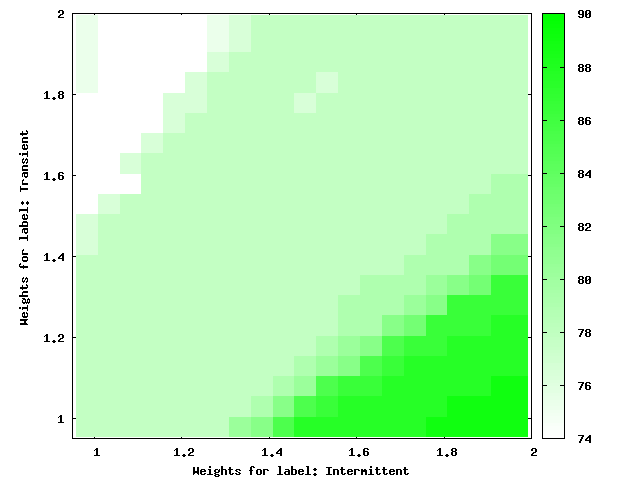
\includegraphics[scale=0.25]{figures/poly256i.png}
                \caption{Transient fault accuracy, polynomial kernel}
        \end{subfigure}

        \begin{subfigure}[h]{0.45\linewidth}
                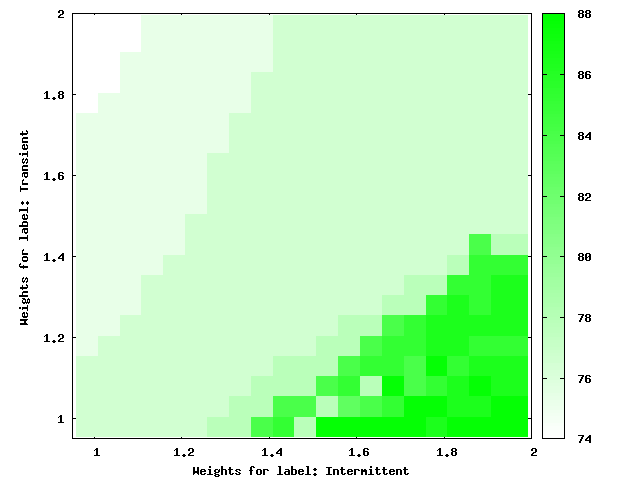
\includegraphics[scale=0.25]{figures/rbf256i.png}
                \caption{Intermittent fault accuracy, RBF kernel}
        \end{subfigure}
			\begin{subfigure}[h]{0.45\linewidth}
                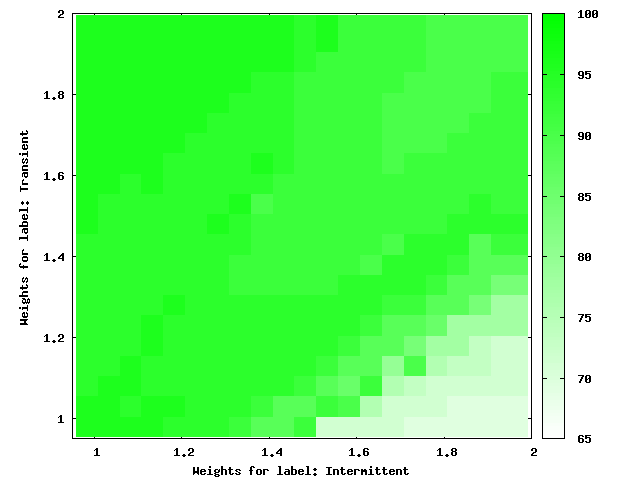
\includegraphics[scale=0.25]{figures/rbf256t.png}
                \caption{Transient fault accuracy, RBF kernel}
        \end{subfigure}

        \begin{subfigure}[h]{0.45\linewidth}
                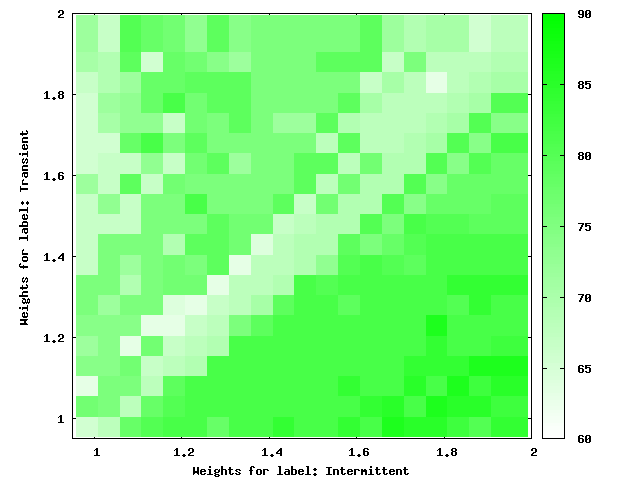
\includegraphics[scale=0.25]{figures/sig256i.png}
                \caption{Intermittent fault accuracy, sigmoid kernel}
        \end{subfigure}
			\begin{subfigure}[h]{0.45\linewidth}
                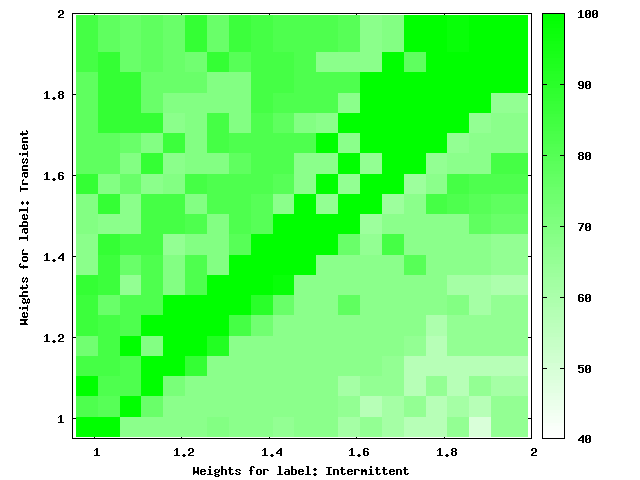
\includegraphics[scale=0.25]{figures/sig256t.png}
                \caption{Transient fault accuracy, sigmoid kernel}
        \end{subfigure}

        \caption{Plots of accuracy by varying class-weights for p256k}
        \label{fig:heatmap} 
\end{figure}



\section{Classification using extrapolation of known training datasets}
So far evaluation of test data is done using a sample population of of the same circuit type. In this section two other possibilities are considered. First, to use a sample population of known circuit type, to classify data of other circuit type. Second, to have a single training dataset, and use a classifier model built from this to predict example data of a circuit type, whose sample population is present in this \emph{universal} dataset.

\subsection{Using single known model for classification}
In practical situations, we might not have the necessary training data for a new product, especially at the start of production. This section explores possibility of extrapolating known datasets for new circuit types. This set of experiments are done using training data of p295k to predict test sets of other circuit types. p295k is chosen as sample population as it provided with relatively most accurate results in first set of experiments. The results obtained are summarized in table~\ref{tab:univ295k}.

\begin{table}[h]
\captionsetup{justification=centering}
\resizebox{\textwidth}{!}{%
\begin{tabular}{cccccc}
\hline
\multirow{3}{*}{Kernel}     & \multirow{3}{*}{Cross-validation accuracy (\%)} & \multirow{3}{*}{Circuit} & \multicolumn{3}{c}{Accuracy (\%)}                             \\ \cline{4-6} 
                            &                                                 &                          & \multicolumn{2}{c}{Intermittent} & \multirow{2}{*}{Transient} \\ \cline{4-5}
                            &                                                 &                          & without noise    & with noise    &                            \\ \hline
\multirow{5}{*}{Linear}     & \multirow{5}{*}{89.17}                          & p45k                     & 77.08            & 72.91         & 95.91                      \\
                            &                                                 & p100k                    & 71.42            & 64.28         & 75.51                      \\
                            &                                                 & p141k                    & 78.57            & 73.08         & 100                        \\
                            &                                                 & p267k                    & 77.5             & 62.5          & 100                        \\
                            &                                                 & p279k                    & 78.94            & 57.89         & 97.95                      \\
\hline
\multirow{5}{*}{Polynomial} & \multirow{5}{*}{90.78}                          & p45k                     & 79.16            & 81.63         & 75.51                      \\
                            &                                                 & p100k                    & 78.57            & 76.19         & 73.46                      \\
                            &                                                 & p141k                    & 88.09            & 80.95         & 91.83                      \\
                            &                                                 & p267k                    & 82.5             & 77.5          & 87.75                      \\
                            &                                                 & p279k                    & 78.94            & 76.31         & 97.95                      \\
\hline
\multirow{5}{*}{RBF}        & \multirow{5}{*}{92.28}                          & p45k                     & 79.16            & 81.25         & 73.46                      \\
                            &                                                 & p100k                    & 78.57            & 73.8          & 71.42                      \\
                            &                                                 & p141k                    & 88.09            & 80.95         & 97.95                      \\
                            &                                                 & p267k                    & 82.5             & 72.5          & 89.79                      \\
                            &                                                 & p279k                    & 78.94            & 71.05         & 100                        \\
\hline
\multirow{5}{*}{Sigmoid}    & \multirow{5}{*}{85.64}                          & p45k                     & 79.16            & 81.25         & 73.46                      \\
                            &                                                 & p100k                    & 78.57            & 73.8          & 71.42                      \\
                            &                                                 & p141k                    & 88.09            & 80.95         & 97.95                      \\
                            &                                                 & p267k                    & 82.5             & 72.5          & 89.79                      \\
                            &                                                 & p279k                    & 78.94            & 71.79         & 100                       \\
\hline
\end{tabular}
}
\caption{Accuracy by extrapolating training dataset of p295k to test other circuits}
\label{tab:univ295k}
\end{table}

Comparison with results from those obtained in section~\ref{sec:wp}, shows an increase in accuracy levels. This can be attributed to two factors, a comparatively balanced dataset of p295k and high cross-validation accuracy levels of this dataset. Hence it is observed that, using a good-quality known dataset, examples from other circuit types can be classified with acceptable accuracy levels.

\subsection{Using a universal training set for classification}

In this set of experiments, a single universal sample population is built using sample populations of individual circuit types. The aim of this experiment to check a possibility of building an incremental universal dataset, which is able to classify data from any of known circuit types. Table~\ref{tab:universal} summarizes results observed.

\begin{table}[h]
\captionsetup{justification=centering}
\resizebox{\textwidth}{!}{%
\begin{tabular}{cccccc}
\hline
\multirow{3}{*}{Kernel}     & \multirow{3}{*}{Cross-validation accuracy (\%)} & \multirow{3}{*}{Circuit} & \multicolumn{3}{c}{Classification accuracy (\%)}              \\ \cline{4-6} 
                            &                                                 &                          & \multicolumn{2}{c}{Intermittent} & \multirow{2}{*}{Transient} \\ \cline{4-5}
                            &                                                 &                          & without noise    & with noise    &                            \\ \hline
\multirow{6}{*}{Linear}     & \multirow{6}{*}{82.84}                          & p45k                     & 66.66            & 64.58         & 100                        \\
                            &                                                 & p100k                    & 66.66            & 61.9          & 89.79                      \\
                            &                                                 & p141k                    & 80.95            & 76.19         & 100                        \\
                            &                                                 & p267k                    & 70               & 65            & 95.91                      \\
                            &                                                 & p279k                    & 71.05            & 60.52         & 97.95                      \\
                            &                                                 & p295k                    & 81.39            & 79.06         & 100                        \\
\hline
\multirow{6}{*}{Polynomial} & \multirow{6}{*}{86.52}                          & p45k                     & 75               & 25            & 95.91                      \\
                            &                                                 & p100k                    & 98.57            & 66.66         & 89.79                      \\
                            &                                                 & p141k                    & 88.09            & 78.57         & 100                        \\
                            &                                                 & p267k                    & 82.5             & 67.5          & 97.95                      \\
                            &                                                 & p279k                    & 76.31            & 63.15         & 100                        \\
                            &                                                 & p295k                    & 93.02            & 81.39         & 95.91                      \\
\hline
\multirow{6}{*}{RBF}        & \multirow{6}{*}{86.58}                          & p45k                     & 79.16            & 77.08         & 89.79                      \\
                            &                                                 & p100k                    & 78.57            & 69.04         & 87.75                      \\
                            &                                                 & p141k                    & 88.09            & 78.57         & 100                        \\
                            &                                                 & p267k                    & 82.5             & 70            & 93.87                      \\
                            &                                                 & p279k                    & 78.94            & 68.42         & 100                        \\
                            &                                                 & p295k                    & 93.02            & 86.04         & 97.95                      \\
\hline
\multirow{6}{*}{Sigmoid}    & \multirow{6}{*}{83.71}                          & p45k                     & 81.25            & 64.58         & 79.59                      \\
                            &                                                 & p100k                    & 83.33            & 66.66         & 83.67                      \\
                            &                                                 & p141k                    & 88.09            & 71.42         & 81.63                      \\
                            &                                                 & p267k                    & 87.5             & 72.5          & 69.38                      \\
                            &                                                 & p279k                    & 81.57            & 60.52         & 79.59                      \\
                            &                                                 & p295k                    & 97.67            & 86.04         & 85.71     \\
\hline                
\end{tabular}
}
\caption{Accuracy using single universal training dataset}
\label{tab:universal}
\end{table}

The universal dataset is also able to classify faults fairly accurately. Using polynomial and RBF kernels, accuracy levels of both intermittent and transient fault classification increased considerably, at the same time. This is mainly because of increase of sample population providing  higher number of positive examples of both classes and eventually resulting in better fitting of hypothesis class. A further increase in accuracy levels, for both or any one of fault types is possible using techniques discussed in section~\ref{sec:ww}.


